\documentclass[a4paper,ngerman]{atseminar}

\usepackage{microtype}
\usepackage{graphicx}
\usepackage{algorithm2e}
\usepackage[left]{lineno}
\usepackage{complexity}
\usepackage{csquotes}
\usepackage{hyperref}
\usepackage{booktabs}
\usepackage{float}

\linenumbers

\newcommand{\N}{\ensuremath{\mathbb{N}}\xspace}
\renewcommand{\A}{\ensuremath{\mathcal{A}}\xspace}
\newcommand{\B}{\ensuremath{\mathcal{B}}\xspace}
\newcommand{\BigO}[1]{\ensuremath{\operatorname{\mathcal{O}}\bigl(#1\bigr)}\xspace}
\newcommand{\BigOStar}[1]{\ensuremath{\operatorname{\mathcal{O*}}\bigl(#1\bigr)}\xspace}
\renewcommand{\deg}[1]{\ensuremath{\operatorname{\triangle}\bigl(#1\bigr)}\xspace}

\newtheorem{observation}[theorem]{\textbf{Beobachtung}}

\newcounter{reductionruleCounter}
\newtheorem{reductionrule}[reductionruleCounter]{\textbf{Reduktionsregel}}

%% Please do not include packages that change the layout/size of the
%% of the document. They will be removed.

\bibliographystyle{plain}%the recommended bibstyle

% Preamble with header information 
\subject{Ausarbeitungen für das Proseminar}
\title{Algorithmen für NP-schwere Probleme}
\titlerunning{Proseminar Algorithmen für NP-schwere Probleme}%optional





%Organizer macros:%%%%%%%%%%%%%%%%%%%%%%%%%%%%%%%%%%%%%%%%%%%%%%%%%%%%%


%% do not use this field, but \summaryauthor
\author{}

%%%%%%%%%%%%%%%%%%%%%%%%%%%%%%%%%%%%%%%%%%%%%%%%%%%%%%%%%%%%%%%%%%%%%%%%%%%%%%%
%%%%%%%%%%%%%%%%%%%%%%%% begin of document %%%%%%%%%%%%%%%%%%%%%%%%%%%%%%%%%%%%
%%%%%%%%%%%%%%%%%%%%%%%%%%%%%%%%%%%%%%%%%%%%%%%%%%%%%%%%%%%%%%%%%%%%%%%%%%%%%%%
\begin{document}

\maketitle

\GERMAN

%%%%% YOUR REPORT BEGINS HERE
\section{Parametrisierte Algorithmen II}
\summaryauthor[Oliver Enes]{Oliver Enes}

\begin{abstract}
Parametrisierte Algorithmen sind ein relativ junges Teilgebiet der theoretischen Informatik und beschäftigen sich mit der
Laufzeitanalyse von Algorithmen. Eine feingranularere Untersuchung im Vergleich zu bisherigen Methoden wird dadurch erzielt,
dass neben der Instanzgröße selbst eine strukturelle Eigenschaft der Instanz -- genannt Parameter -- mit in die Laufzeitanalyse einbezogen wird.
Durch passende Wahl des Parameters lässt sich dabei ein Indikator für die \enquote{Schwierigkeit} eines Problems schaffen.
Die vorliegende Ausarbeitung gibt einen groben Überblick über das Thema.
Dabei wird ausgehend von der formalen Definition eines parametrisierten Problems die parametrisierte Komplexitätsklasse \FPT\xspace und
die Methodik der Problemkerne und Problemkernreduktion eingeführt. Es wird die Äquivalenz von \FPT-Problemen sowie Problemen mit Problemkern gezeigt und
eine konkrete Problemkernreduktion am Beispiel des Problems \textsc{VertexCover} durchgeführt.
Zusätzlich werden Probleme eingeführt, für die kein \FPT-Algorithmus bekannt ist. Mit der parametrisierten Reduktion
und dem Begriff der \W{[1]}-Härte wird eine Methodik zur Reduktion parametrisierter Probleme auf andere Probleme gezeigt, die genutzt werden kann, um die geringe Wahrscheinlichkeit für die Existenz von \FPT-Algorithmen für
bestimmte Probleme zu zeigen.
Abschließend werden mit der Exponential Time Hypothesis (ETH) und der Strong Exponential Time Hypothesis (SETH) zwei unbewiesene
Annahmen an die Laufzeit eines Problems bzw. einer Familie von Problemen vorgestellt, die dazu genutzt werden können,
untere Schranken an die Laufzeit von Algorithmen zu formulieren, die mit vielen Laufzeiten existierender State-of-the-Art-Algorithmen
übereinstimmen. Die Anwendung von ETH und SETH wird an einer Reihe von Beispielen verdeutlicht.
\end{abstract}

\subsection{Einleitung}

Parametrisierte Algorithmen ermöglichen im Vergleich zur klassischen Komplexitätstheorie eine feinere Untersuchung der Laufzeit eines \NP-schweren Problems.
Dazu wird die Laufzeit eines Algorithmus nicht nur in der Eingabegröße, sondern zusätzlich in einem \textbf{Parameter} betrachtet.
Der Parameter ist eine Kenngröße der Probleminstanz (z.B. chromatische Zahl bei Graphen) und formalisiert die Schwierigkeit einer Probleminstanz.

\noindent
Das Konzept des Parameters motiviert die Erweiterung des Problembegriffs zum \textbf{parametrisierten Problem}:

\begin{definition}[Parametrisiertes Problem]
  Sei $\Sigma$ ein endliches Alphabet.

  \noindent
  Ein \textbf{parametrisiertes Problem} ist eine Sprache $L \subseteq \Sigma^* \times \N$.
  \noindent
  Die zweite Komponente einer Probleminstanz $I \in L$ wird als \textbf{Parameter} bezeichnet.
\end{definition}

\noindent
Ein Problem wird durch das Festlegen eines Parameters zum parametrisierten Problem:

\begin{table}[H]
  \centering
  \caption{Beispiele für parametrisierte Probleme}
  \begin{tabular}{ll}
    \toprule
    \textbf{Problem} & \textbf{Parameter} \\
    \midrule
    \textsc{VertexCover} & Größe des Vertex Cover \\
    \midrule
    \textsc{Subset Sum} & Summe aller Elemente \\
    \midrule
    \textsc{3Color} & größte Cliquengröße \\
    \midrule
    \textsc{VertexCover} &  minimaler Knotengrad \\
    \bottomrule
    
  \end{tabular}
  \end{table}

\noindent
Es sei darauf hingewiesen, dass die Parameterwahl nicht eindeutig ist. Oft wird die Lösungsgröße gewählt.

\noindent
Während der Begriff des parametrisierten Problems unabhängig von \NP-Schwierigkeit ist, kommt diesem eine besondere
Bedeutung im Zusammenhang mit der Laufzeitanalyse \NP-schwerer Probleme zu: Laufzeiten lassen sich nun nicht nur in der Eingabegröße, sondern zusätzlich
im Parameter analysieren.
Dies begründet neue Komplexitätsklassen. Dabei ist eine für uns von zentralem Interesse:

\begin{definition}[Problemklasse \FPT]
  \label{OE:def:fpt}
  Ein parametrisiertes Entscheidungsproblem heißt \textbf{FPT (Fixed-Parameter-Tractable)}, wenn ein Algorithmus existiert,
  der alle Probleminstanzen $(x, k)$ mit Laufzeit \BigO{f(k) \cdot |x|^c} löst.
  Dabei ist $c \in \N$ und $f: \N \rightarrow \N$ eine beliebige berechenbare Funktion.
\end{definition}

\begin{example}[FPT-Laufzeiten]
  $ $
  \begin{itemize}
    \item \BigO{2^k \cdot (|x|^3+42|x|)}
    \item \BigO{(43k^2+k) \cdot {|x|^2}}
    \item \BigO{|x|^{123}+12}
    \item \BigO{\varphi(k, k - 5, k - \sqrt{k}) \cdot \log(|x| + 1)} wobei $\varphi$ die Ackermann-Funktion ist.
  \end{itemize}
\end{example}

\noindent
Die Laufzeit ist also insbesondere polynomiell in der Instanzgröße und nahezu beliebig im Parameter.
Lässt sich also für ein parametrisiertes Entscheidungsproblem ein \FPT-Algorithmus finden, so kann dieser höchstens im Parameter superpolynomiell sein.
Dabei wird eine wünschenswerte Eigenschaft des Parameters deutlich: der Parameter formalisiert die \enquote{Gutartigkeit} einer Probleminstanz, indem er den potentiellen superpolynomiellen
Anteil der Laufzeit beschränkt. Dabei sei angemerkt, dass die Parameterwahl zentral für diese Eigenschaft ist.
So kann für das gleiche \enquote{klassische} Problem als parametrisiertes Problem in einem Parameter ein \FPT-Algorithmus existieren, während für eine andere Wahl
des Parameters kein solcher Algorithmus bekannt ist.

\noindent
Oft interessiert man sich nur für den Anteil der Laufzeit, der vom Parameter abhängt. In diesem Fall lässt sich vereinfacht
$\BigOStar{f(k)}$ schreiben, um eine \FPT-Laufzeit zu formulieren, dessen polynomieller Anteil beliebig ist.
Es ist also $\BigOStar{f(k)} = \bigcup_{c \in \N} \BigO{f(k) \cdot |x|^c}$.

\subsection{Problemkerne und Problemkernreduktion}
\label{OE:sec:kernel}

Eine wichtige Technik im Bereich der parametrisierten Algorithmen ist die Bildung von Problemkernen.
Ein Problemkern entsteht, indem eine gegebene Instanz eines parametrisierten Problems derart reduziert wird, dass der in polynomieller Zeit lösbare
Teil der Instanz entfernt wird, sodass die so entstehende Instanz nur noch den Teil enthält, dessen Lösung mit bekannten Algorithmen superpolynomielle Zeit beansprucht.
\noindent
Dabei fordern wird jedoch, dass die Größe des Problemkerns nur vom Parameter abhängt.
Formal ergibt sich das Konzept der Problemkerne und der Problemkernreduktion.

\begin{definition}[Problemkerne und Problemkernreduktion]
  \label{OE:def:kernel}
  Sei $L  \subseteq \Sigma^* \times \N$ ein parametrisiertes Problem.
  Eine Problemkernreduktion $ \Phi: \Sigma^* \times \N \rightarrow \Sigma^* \times \N $ ist eine Funktion, sodass:
  \begin{itemize}
      \item $I \in L \iff I' := \Phi(I) \in L $ (\textbf{Äquivalenz})
      \item $|I'| \leq f(k)$ für eine beliebige Funktion $f: \N \rightarrow \N$ (\textbf{Beschränktheit})
      \item $\Phi$ ist polynomiell in $|x| + k$ berechenbar (\textbf{Berechenbarkeit})
  \end{itemize}

  \noindent
  $I'$ heißt \textbf{Problemkern} von $I$.
\end{definition}

\noindent
Es sei darauf hingewiesen, dass $\Phi$ nicht nur in $|x|$, sondern auch in $k$ polynomiell berechenbar sein muss.
Dies lässt sich einsehen durch folgende Beobachtung:
\begin{observation}

  Eine parametrisierte $k$-\textsc{VertexCover} Instanz, wobei die Lösungsgröße der Parameter ist, lässt sich mittels eines
  Bruteforce Algorithmus $\mathcal{A}$ in $\BigO{\binom{n}{k} \cdot m} \preceq \BigO{n^k \cdot m}$ lösen.

  \noindent
  Entsprechend lässt sich eine Reduktion $\tilde{\Phi}$ konstruieren, die Instanzen mittels $\mathcal{A}$ löst und dann triviale
  Problemkerne zurückgibt.
  Dann gelten (\textbf{Äquivalenz}) und (\textbf{Beschränktheit}), jedoch hat $\tilde{\Phi}$ exponentielle Laufzeit in $k$.
  \noindent
  Durch die Aufweichung der Laufzeit-Bedingung ist es also möglich, Reduktionen zu konstruieren, die auch \enquote{schwere} Teile einer Instanz lösen.
  Dies widerspricht der Idee eines Problemkerns, der eben die Teile einer Instanz enthält, die superpolynomielle Laufzeit verursachen.
  Unabhängig davon, birgt eine derartige Aufweichung der Laufzeit auch im praktischen Einsatz Nachteile: Wenn die Problemkernreduktion selbst
  schon exponentielle Laufzeit benötigt, besteht oft kein großer Sinn, zuerst einen Problemkern zu berechnen und diesen dann in superpolynomieller Zeit
  zu lösen.
\end{observation}

\noindent
Ein gängiges Vorgehen ist also, zunächst einen -- möglichst kleinen -- Problemkern in polynomieller Zeit zu berechnen, dessen Lösung zwar tendenziell exponentiell viel Zeit benötigt,
durch die Größe des Problemkerns aber im Vergleich zur ursprünglichen Instanz in guter Zeit gelöst werden kann.

\noindent
Wir wollen die Bildung eines Problemkerns exemplarisch am Problem \textsc{VertexCover} verdeutlichen. Dieses definieren wir als
parametrisiertes Entscheidungsproblem $k$-\textsc{VertexCover}:

\begin{definition}[Problem $k$-\textsc{VertexCover}]
  $ $\newline
  \begin{tabular}{ll}
    \textbf{Gegeben:} & Einfacher, ungerichteter Graph  $G = (V, E), \quad k \in \N$ \\
    \textbf{Parameter:} & Lösungsgröße $k$ \\
    \textbf{Frage:} & Existiert $M \subseteq V$, sodass $ |M| \leq k $ und $ \forall e \in E : e \cap M \neq \emptyset$?
  \end{tabular}
\end{definition}

\begin{example}[Problemkernreduktion für k-\textsc{VertexCover} \cite{Beyond}]
    Die Problemkernreduktion besteht aus einer Reihe sogenannter Reduktionsregeln. Dabei handelt es sich um eine von anderen Reduktionsregeln unabhängige
    Vorschrift, wie eine Instanz in eine andere überführt wird.
    Wichtig ist, neben der polynomiellen Laufzeit, die sogenannte Äquivalenzbedingung (im Englischen oft als \enquote{safeness} bezeichnet).
    Diese fordert, dass eine reduzierte Instanz genau dann eine Ja-Instanz ist, wenn die ursprüngliche Instanz eine Ja-Instanz ist.
    Hingegen ist die Beschränktheit der Instanzgröße durch den Parameter nicht gefordert.

    \begin{reductionrule}[\cite{Beyond}]
      \label{OE:reduction:1}
      Ist $(G, k)$ eine $k$-\textsc{VertexCover} Instanz und $U \subseteq V(G)$, sodass $ (U \times V(G)) \cap E(G) = \emptyset $ ist, so ist $(G - U, k)$
      eine äquivalente Instanz.
    \end{reductionrule}
    \begin{proof}
      $U$ ist eine Menge an isolierten Knoten in $G$. Diese tragen nichts zur Kantenabdeckung bei.
    \end{proof}

    \begin{reductionrule}[\cite{Beyond}]
      \label{OE:reduction:2}
      Ist $(G, k)$ eine k-\textsc{VertexCover} Instanz und $v \in V(G)$ mit Grad $\deg{v} \geq k + 1$,
      so ist $(G - v, k - 1)$ eine äquivalente Instanz und $v$ im Vertex Cover $M$ von $G$ enthalten.
    \end{reductionrule}
    \begin{proof}
      Dass $v$ in M enthalten ist, zeigen wir wie folgt:
      Angenommen, $v \notin M$. Dann muss die Nachbarschaft $N(v)$ in M enthalten sein. Jedoch ist $|N(v)| = \deg{v} \geq k + 1 > k$.


      \noindent
      Die Äquivalenz der Instanzen sieht man folgendermaßen ein:

      \noindent
      Ist $(G, k)$ eine Ja-Instanz mit Vertex Cover $M$ und $v \in V(G)$ mit $\deg{v} \geq k + 1$, so ist $M' := M \backslash \{v\}$ ein Vertex Cover in $G - v$.
      Insbesondere ist $|M'| = |M| - 1 \leq k -1$.
      Damit löst $M'$ die reduzierte Instanz $(G - v, k - 1)$.

      \noindent
      Sei nun $(G - v, k - 1)$ eine reduzierte $k$-\textsc{VertexCover} Instanz mit Lösung $M'$. Durch die Hinzunahme von $v$ entsteht der Graph $G$.
      Alle neu hinzukommenden Kanten werden durch den Knoten $v$ abgedeckt.
      Damit ergibt sich als Vertex Cover für $G$ die Menge $M := M' \cup \{v\}$.
      Es ist $|M| = |M'| + |\{v\}| = |M'| + 1 \leq k$. Damit löst $M$ die Instanz $(G, k)$.
    \end{proof}

    \noindent
    Durch Anwendung von der \hyperref[OE:reduction:2]{2. Reduktionsregel} können isolierte Knoten entsehen. Diese können wiederum mit Hilfe der \hyperref[OE:reduction:3]{3. Reduktionsregel} entfernt
    werden.
    Reduktionsregeln können (und sollten) also mehrmals angewandt werden. Lässt sich eine Reduktionsregel nicht mehr anwenden, selbst nachdem andere Reduktionsregeln
    die Instanz weiter reduziert haben, sagt man, dass die Reduktionsregel \textbf{erschöpfend} angewandt worden ist.

    \noindent
    Wir kommen zur letzten Reduktionsregel:

    \begin{reductionrule}[\cite{Beyond}]
      \label{OE:reduction:3}
      Ist $(G, k)$ eine k-\textsc{VertexCover} Instanz mit $\deg{v} \leq k$ für alle $ v \in V(G)$ und $|E(G)| > k^2$, so ist $(G, k)$
      eine Nein-Instanz. Es wird eine triviale Nein-Instanz zurückgegeben. 
    \end{reductionrule}
    \begin{proof}
      Wir zeigen, dass eine Menge an $k$ Knoten nicht ausreichen kann, um alle Kanten in $G$ abzudecken.
      \noindent
      Maximale Abdeckung wird erreicht, wenn die abgedeckten Kantenmengen der einzelnen Knoten in $M$ disjunkt sind und der Grad aller Knoten maximal ist.
      
      \noindent
      Dann lassen sich $\sum_{v \in M}{\deg{v}} = \sum_{v \in M}{k} = k^2$ Kanten abdecken.
      \noindent
      Da aber $|E(G)| > k^2$, kann folglich kein Vertex Cover der Größe $k$ existieren.
    \end{proof}
    Es sei angemerkt, dass, obwohl im Falle $|E(G)| > k^2$ bereits die Lösung der gegebenen Instanz bekannt ist, wir trotzdem eine sogenannte triviale Instanz
    und nicht die Lösung selbst zurückgeben. Dabei handelt sich um reinen Formalismus: Reduktionsregeln reduzieren gegebene Instanzen in
    andere \textbf{Instanzen}. Daher geben wir einfach eine Instanz zurück, der man die Lösung \enquote{direkt ansehen} kann.

    \noindent
    Alle Reduktionsregeln sind in \hyperref[OE:fig:reductionRules]{Abbildung }\ref{OE:fig:reductionRules} grafisch verdeutlicht.

    \begin{figure}[h]
      \centering
      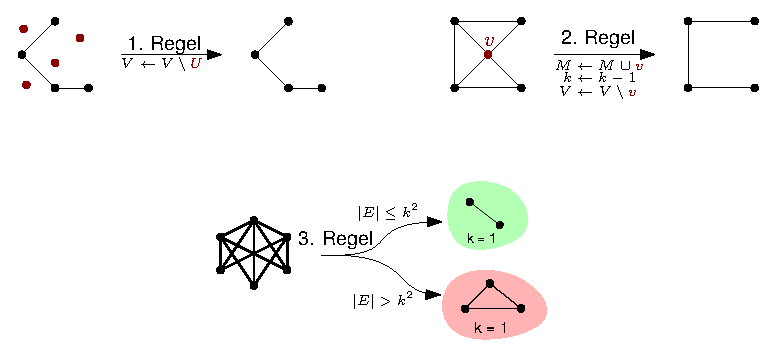
\includegraphics[scale = 1.0]{./images/reduction-rules.eps}
      \caption{Reduktionsregeln für $k$-\textsc{VertexCover}.}
      \label{OE:fig:reductionRules}
     \end{figure}
    
    \noindent
    Jede der hier aufgeführten Reduktionsregeln kann in polynomieller Zeit angewendet werden. Uns interessiert nun die Größe einer
    Instanz, die nach erschöpfender Anwendung aller Reduktionsregeln entsteht. Unsere Hoffnung ist, dass die Reduktionen eine Instanz derart
    verkleinern, dass deren Größe nur noch vom Parameter abhängt. Dann bildet die erschöpfende Anwendung unserer Reduktionsregeln die
    Problemkernreduktion.
    Tatsächlich erhalten wir folgenden Problemkern:
    \begin{theorem}[Problemkern für $k$-\textsc{VertexCover} \cite{Beyond}]
      Eine $k$-\textsc{VertexCover} Instanz reduziert sich nach erschöpfender Anwendung der Reduktionsregeln \ref{OE:reduction:1}, \ref{OE:reduction:2}, \ref{OE:reduction:3} auf
      eine Größe in \BigO{k^2}.
    \end{theorem}
    \begin{proof}
      Sei $\tilde{G}$ der Graph, der aus einer $k$-\textsc{VertexCover} Instanz $(G, k)$ nach erschöpfender Anwendung der Reduktionsregeln \ref{OE:reduction:1}, \ref{OE:reduction:2} und \ref{OE:reduction:3} entstanden ist.

      \noindent
      Dann besitzt $\tilde{G}$ nach der \hyperref[OE:reduction:1]{1. Reduktionsregel} keine isolierten Knoten mehr. Das heißt, jeder Knoten ist zu mindestens einer
      Kante inzident.
      Nach Anwendung der \hyperref[OE:reduction:2]{2. Reduktionsregel} hat jeder Knoten maximalen Grad $k$.
      Damit lässt sich die \hyperref[OE:reduction:3]{3. Reduktionsregel} anwenden, die eine Instanz mit maximal $k^2$ vielen Kanten
      hervorbringt.
      Dann hat $\tilde{G}$ maximal $2k^2$ viele Knoten.
    \end{proof}

    \noindent
    Erfreulicherweise ist der Problemkern sogar polynomiell groß. Dies ist im Allgemeinen nicht so und im Fall eines polynomiellen
    Problemkerns für ein \NP-vollständiges Problem hat -- unter der Vorraussetzung $\P \neq \NP$ -- jeder Algorithmus, der den Problemkern löst, exponentielle Laufzeit.
\end{example}

\subsection{\FPT\xspace und Problemkerne}

Die weiter oben erwähnte \hyperref[OE:def:fpt]{\FPT-Laufzeit} sowie \hyperref[OE:sec:kernel]{Problemkerne} hängen stark miteinander zusammen:

\begin{theorem}[FPT-Laufzeit und Problemkerne \cite{Beyond}]
  Ein entscheidbares parametrisiertes Problem besitzt genau dann einen Problemkern, wenn es in \FPT\xspace ist.
\end{theorem}
\begin{proof}
    Sei zunächst $I = (x, k)$ eine Instanz eines entscheidbaren parametrisierten Problems $L$ mit Problemkern. Dann existiert eine Problemkernreduktion
    $\Phi$. Da $L$ entscheidbar ist, existiert auch ein Algorithmus \A, der $L$ entscheidet.
  
    \noindent
    Wir konstruieren nun einen \FPT-Algorithmus wie folgt:
    Zunächst erzeugen wir den Problemkern $(x', k') := \Phi(I)$. Für diesen gilt nach Definition $|I'| \leq g(k)$ für eine berechenbare Funktion
    $g: \N \rightarrow \N$. Wir lassen \A den Problemkern $I'$ entscheiden.
  
    \noindent
    Die Laufzeit setzt sich zusammen aus der Laufzeit für die Problemkernbildung und der Laufzeit $f: \N \rightarrow \N$ von \A:
    \BigO{(|x| + k)^c + f(g(k))} $\preceq$ \BigO{f(g(k)) \cdot |x|^c}. 
    Damit ist $L$ in \FPT.

    \vspace{0.25cm}
    \noindent
    Sei nun $I = (x, k)$ eine Instanz eines entscheidbaren \FPT\xspace Problems $L$.
    Dann existiert ein Algorithmus \A mit Laufzeit \BigO{f(k) \cdot |x|^c}.

    \noindent
    Wir unterscheiden zwei Fälle:
    Im ersten Fall sei $|x| > f(k)$. Dann hat \A eine Laufzeit in \BigO{|x|^{c+1}}. Löse die Instanz mit \A und gib die Lösung
    als triviale Instanz zurück. Die Laufzeit ist dominiert durch \A und damit polynomiell in $|x| + k$.
    
    \noindent
    Im zweiten Fall ist $|x| \leq f(k)$. Damit ist $|x|$ durch k beschränkt und somit $I$ selbst schon ein Problemkern (vgl. Definition \ref{OE:def:kernel}).
    Es wird $I$ zurückgegeben.
  \end{proof}

  \noindent
  Es sei angemerkt, dass obwohl die Methodik, wie in der letzten Hälfte des Beweises angemerkt, einen gültigen Problemkern erzeugt, dieser
  keinesfalls minimal ist \cite{Beyond}.

\subsubsection{Prametrisierte Reduktionen}

Eine zentrale Technik um zu zeigen, dass ein Problem \NP-schwer ist,
ist die polynomielle Many-one-Reduktion.
Dabei werden in polynomieller Zeit Instanzen eines Problems $L$ auf Instanzen eines Problems $L'$ reduziert.
Ist folglich ein Algorithmus für $L'$ bekannt, lässt sich $L$ durch Reduktion auf $L'$ lösen.
Wäre also $L$ ein \NP-schweres Problem, folgt durch die Reduktion, dass $L'$ auch \NP-schwer ist.
Dabei muss die Laufzeit der Reduktion polynomiell sein.

\noindent
Wir möchten uns nun ein ähnliches Konzept für parametrisierte Probleme ansehen: die parametrisierte Reduktion
(auch als \FPT-Reduktion bekannt).

\begin{definition}[Parametrisierte Reduktion]
  Seien $L, L' \subseteq \Sigma^* \times \N$ zwei parametrisierte Probleme.
  Eine \textbf{Problemkernreduktion $g: \Sigma^* \times \N \rightarrow \Sigma^* \times \N$} reduziert eine Instanz
  von $L$ auf eine Instanz von $L'$, wenn gilt:
  \begin{itemize}
    \item $I:= (x, k) \in L \Leftrightarrow I' := (x', k') :=g(I) \in L'$. \quad (\textbf{Äquivalenz})
    \item $k' \leq h(k)$ für beliebiges $h: \N \rightarrow \N$. \quad (\textbf{Parametrisierung})
    \item $g$ ist berechenbar und die Laufzeit ist in \FPT. \quad (\textbf{Berechenbarkeit})
  \end{itemize}

  Wir schreiben $L \propto_{FPT} L'$.
\end{definition}

\noindent
Eine parametrisierte Reduktion unterscheidet sich von der \enquote{klassischen} Many-one-Reduktion folglich darin,
dass diese zusätzlich die Parametrisierung erhält und die Laufzeit in \FPT\xspace ist.
Damit stellt die parametrisierte Reduktion echt stärkere Anforderungen als die Many-one-Reduktion.
Es lassen sich \NP-schwere Probleme finden, die zwar Many-one-reduzierbar auf ein anderes \NP-schweres Problem sind, für die jedoch
keine parametrisierte Reduktion auf selbiges bekannt ist.
Damit wird die Problemklasse \NP\xspace weiter unterteilt: Es bildet sich die \W-Hierarchie \cite{DowneyFellows}, die wir hier aber nicht weiter betrachten werden.
%Es sei für weitere Informationen auf (TODO: Downey Fellows Literatur) verwiesen.

\noindent
Eine Anwendung der parametrisierten Reduktion besteht darin, zu zeigen, dass ein gegebenes parametrisiertes Problem wahrscheinlich keinen
Algorithmus mit \FPT-Laufzeit besitzt.
Dies ist explizit kein formaler Beweis für die Nicht-Existenz eines solchen Algorithmus. Es wird schlichtweg das Argument geführt,
dass eine Lösung des Problems eine Lösung für ein anderes Problem impliziert, welches zuvor trotz hoher Anstrengung von einer Vielzahl
an Menschen nicht gelöst werden konnte.
Dies könnte unter Umständen einen wissenschaftlichen Durchbruch darstellen, der unwahrscheinlich -- aber eben nicht unmöglich -- ist. 

\noindent
Als konkretes Beispiel wollen wir das Problem $k$-\textsc{Clique} betrachten:

\begin{definition}[$k$-\textsc{Clique}]
  $ $\newline
  \begin{tabular}{ll}
    \textbf{Gegeben:} & Einfacher, ungerichteter Graph  $G = (V, E), \quad k \in \N$ \\
    \textbf{Parameter:} & Lösungsgröße $k$ der Clique. \\
    \textbf{Frage:} & Existiert $M \subseteq V$, sodass $ |M| = k $ und $ \forall u, v \in M : \{u, v\} \in E$?
  \end{tabular}
\end{definition}

\noindent
Wir redzuieren $k$-\textsc{Clique} auf $k$-\textsc{IndependentSet}:

\begin{definition}[$k$-\textsc{IndependentSet}]
  $ $\newline
  \begin{tabular}{ll}
    \textbf{Gegeben:} & Einfacher, ungerichteter Graph  $G = (V, E), \quad k \in \N$ \\
    \textbf{Parameter:} & Lösungsgröße $k$ des Independent Set. \\
    \textbf{Frage:} & Existiert $M \subseteq V$, sodass $ |M| = k $ und $ \forall u, v \in M : \{u, v\} \not\in E$?
  \end{tabular}
\end{definition}

\noindent
Sei also $I = (G, k)$ eine $k$-\textsc{Clique} Instanz. Wir betrachten den Komplementärgraph $G^\complement$.
Dann ist $M$ genau dann ein Vertex Cover in $G$, wenn M ein Independent Set in $G^\complement$ ist.
Der Parameter bleibt unverändert und die Konstruktion von $G^\complement$ ist in polynomieller Zeit möglich. 
Es ist also $k$-\textsc{Clique} $\propto_{FPT}$ $k$-\textsc{IndependentSet}. Außerdem sieht man analog \\$k$-\textsc{IndependentSet} $\propto_{FPT} k$-\textsc{Clique} ein.
Folglich sind die Probleme \enquote{parametrisiert äquivalent schwer}.
Für das Problem $k$-\textsc{Clique} ist kein \FPT\xspace Algorithmus bekannt. Wir nehmen dies zum Anlass, $k$-\textsc{Clique} als \enquote{parametrisiert schwerer} als
\FPT-Probleme wie z.B.\\ $k$-\textsc{VertexCover} zu sehen und definieren daher die Problemklasse \W[1]:

\begin{definition}[Problemkasse \W{[}1{]} und \W{[}1{]}-Härte]
  Ein parametrisiertes Problem $L$ ist genau dann in der Problemklasse W{[}1{]}, wenn es parametrisiert reduzierbar auf $k$-\textsc{Clique} ist.
  $L$ ist genau dann \W{[}1{]}-hart, wenn für alle $L' \in \W[1]$ gilt: $L' \propto_{FPT} L$.
\end{definition}
\noindent
Dank der Transitivität der parametrisierten Reduktion reicht es auch, ein \W{[}1{]}-hartes Problem auf das Zielproblem zu reduzieren, um
\W{[}1{]}-Härte zu zeigen.

\noindent
Die Problemklasse \W{[}1{]} ist also über ein kanonisches Problem definiert. Wie die Schreibweise es bereits vermuten lässt,
gibt es auch die Problemklassen $\W[2],\xspace\W[3], \dots$, die zusammen die \W-Hierarchie \cite{DowneyFellows} bilden. Die formale Definition erfolgt über
ein alternatives kanonisches Problem, bei dem die konkrete Wahl der Problemparameter die einzelnen Problemklassen begründet.
Es handelt sich konkret um das Problem \textsc{Weighted Circuit Satisfiability} \cite{DowneyFellows}, welches wir aber nicht weiter betrachten werden.% Es sei an (TODO: Downey Fellows) verwiesen.

\noindent
Wir wollen an dieser Stelle nur zeigen, dass es tatsächlich Probleme gibt, die nicht in \W{[}1{]}  enthalten sind (unter der Annahme $\P \neq \NP$):
Dazu stellen wir zunächst fest, dass sich $k$-\textsc{Clique} mittels eines Bruteforce Ansatzes in $\BigO{\binom{n}{k} \cdot k^2} \preceq \BigO{n^k \cdot k^2}$ lösen lässt.

\noindent
Wir betrachten nun das Problem $k$-\textsc{Color}:

\begin{definition}[$k$-\textsc{Color}]
  $ $\newline
  \begin{tabular}{ll}
    \textbf{Gegeben:} & Einfacher, ungerichteter Graph  $G = (V, E), \quad k \in \N$ \\
    \textbf{Parameter:} & verfügbare Anzahl Farben $k$. \\
    \textbf{Frage:} & Existiert Färbung $c: V \rightarrow \N$ mit $|c(V)| \leq k$ und $(u, v) \in E \Rightarrow c(u) \neq c(v)$?
  \end{tabular}
\end{definition}

\noindent
Um $k$-\textsc{Color} $\not\in \W[1]$ zu zeigen, nehmen wir an, es gälte $k$-\textsc{Color} $\propto_{FPT} k$-\textsc{Clique}.
Dann ließe sich $k$-\textsc{Color} in $\BigO{n^{g(k)}\cdot g(k)^2}$ lösen. Insbesondere lässt sicht dann 3-\textsc{Color} in $\BigO{n^{g(3)} \cdot g(3)^2}$, also in polynomieller Zeit lösen.
Durch die \NP-Vollständigkeit von 3-\textsc{Color} folgt $\P = \NP$.
Der Umstand, dass ein parametrisiertes Problem für einen festen Parameter \NP-hart ist, wird als para-\NP-Härte bezeichnet:

\begin{definition}[para-\NP-Härte]
  Ein parametrisiertes Problem L ist \textbf{para-\NP-hart}, wenn für beliebigen aber festen Parameter $k$ das Problem
  $L_k := \{x | (x, k) \in L\}$ \NP-hart ist.
\end{definition}


\subsection{ETH und SETH}

In diesem Abschnitt beschäftigen wir uns mit zwei unbewiesenen Hypothesen, die untere Schranken für die Laufzeiten für ein bestimmtes Problem bzw. für eine
Familie an Problemen postulieren.
Diese Hypothesen resultieren aus der jahrenlangen vergeblichen Suche nach einem Polynomialzeitalgorithmus für das SAT-Problem \cite{Parameterized, Beyond}.
Nimmt man diese Hypothesen an, lassen sich für viele Probleme untere Schranken für die Laufzeit finden, die mit vielen State-of-the-Art-Algorithmen übereinstimmen \cite{Parameterized, Beyond}.
\noindent
Bei den Hypothesen handelt es sich um die Exponential Time Hypothesis (ETH) und Strong Exponential Time Hypothesis (SETH). Beide sagen etwas über die
Laufzeit des p-\textsc{CNF-SAT}-Problems aus:

\begin{definition}[Problem p-\textsc{CNF-SAT}]
  $ $\newline
  \begin{tabular}{ll}
    \textbf{Gegeben:} & Variablenmenge $V$, Klauselmenge $C$ mit maximal $p \in \N$ Literalen in jeder Klausel. \\
    \textbf{Frage:} & Existiert eine erfüllende Wahrheitsbelegung?
  \end{tabular}
\end{definition}

\noindent
Das \enquote{CNF} im Problemnamen steht für konjunktive Normalform. Die durch die Klauseln gegebene aussagenlogische Formel ist folglich in konjunktiver Normalform gegeben.
ETH und SETH sagen nun folgendes aus:

\begin{definition}[Exponential Time Hypothesis (ETH)]
  \label{oe:definition:eth}
  3-\textsc{CNF-SAT} lässt sich nicht in \BigO{2^{o(|V|)}} lösen.
\end{definition}

\begin{definition}[Strong Exponential Time Hypothesis (SETH)]
  Für jedes feste $\varepsilon < 1$ existiert $p = p(\varepsilon)$, sodass sich p-\textsc{CNF-SAT} nicht in $\BigO{(2 - \varepsilon)^{|V|}} = \BigO{2^{|V|(1 - \varepsilon)}}$ lösen lässt.
\end{definition}
  
\noindent
Nimmt man diese Hypothesen an, ist es möglich, daraus bestimmte Laufzeiten für andere Probleme abzuleiten: Wollen wir zeigen, dass es für ein Problem keinen Algorithmus mit einer bestimmten Laufzeit geben kann
(unter Annahme der Hypothesen!), reduzieren wir 3-\textsc{CNF-SAT} bzw. p-\textsc{CNF-SAT} auf das Problem und zeigen, dass eine Laufzeit für eines der Probleme
entsteht, die der entsprechenden Hypothese widerspricht.

\noindent
Bevor wir uns Beispiele ansehen, sei angemerkt, dass ETH und SETH keine Parametrisierung des Problems voraussetzen. So wird in den ersten Beispielen die Many-one-Reduktion benutzt.
Konkret nutzen wir folgende Aussage:


\begin{theorem}[Sipser (1996) \cite{sipser}]
  \label{oe:theorem:sipser}
  \textsc{3-\textsc{CNF-SAT}} lässt sich auf \textsc{VertexCover} reduzieren.
                Aus einer \textsc{3-\textsc{CNF-SAT}}-Instanz $(V, C)$ wird die \textsc{VertexCover}-Instanz $G$.
                \\
                Es gilt:
                \begin{itemize}
                    \item $|V(G)| = 2|V| + 3|C| $.
                    \item $|M| \leq |V(G)|$ für jedes \textsc{VertexCover} $M$.
                \end{itemize}
\end{theorem}
%Für den Beweis sei auf (TODO Sipser Buch) verwiesen.

\noindent
Mithilfe des Theorems \ref{oe:theorem:sipser} und der \hyperref[oe:definition:eth]{ETH} ergibt sich folgendes Korollar:

\begin{corollary}[\cite{Beyond}]
  Unter Annahme der ETH existiert kein Algorithmus für \textsc{VertexCover} mit Laufzeit in \BigO{2^{o(|V(G)|^{\frac{1}{3}})}}.
\end{corollary}
\begin{proof}
  Sei $I = (V, C)$ eine 3-\textsc{CNF-SAT} Instanz. Wir lösen $I$ indem wir mit Hilfe des \hyperref[oe:theorem:sipser]{Theorems} \ref{oe:theorem:sipser}
  $I$ auf eine \textsc{VertexCover} Instanz $I' = (G, k)$ reduzieren.

  \noindent
  Angenommen, es gäbe einen Algorithmus für \textsc{VertexCover} mit Laufzeit \BigO{2^{o(|V(G)|^{\frac{1}{3}})}}.
  Dann ergibt sich im Widerspruch zur \hyperref[oe:definition:eth]{ETH} ein Algorithmus für 3-\textsc{CNF-SAT} mit folgender Laufzeit:
  $2^{o(|V(G)|^{\frac{1}{3}})} \preceq 2^{o((2|V| + 3|C|)^{\frac{1}{3}})} \preceq 2^{o((2|V| + |V|^3)^{\frac{1}{3}})} \preceq 2^{o(|V|)}$.
  Dabei folgt die vorletzte Ungeleichung, da es bei $|V|$ verschiedenen Variablen und einer Klauselgröße von drei maximal $|V|^3$ Klauseln geben kann.
\end{proof}

\noindent
Unter Annahme der \hyperref[oe:definition:eth]{ETH} lassen sich noch stärkere Aussagen zeigen.
Diese können wiederum genutzt werden, um bestimmte Laufzeiten anderer Algorithmen auszuschließen.
Eine solche Aussage liefert die Arbeit von Impaglioazzo et al.:

\begin{theorem}[Impaglioazzo et al. (2001) \cite{impagliazzo}]
  \label{oe:theorem:impaglioazzo}
  Unter Annahme der \hyperref[oe:definition:eth]{ETH} hat 3-\textsc{CNF-SAT} keinen Algorithmus mit Laufzeit $\BigO{2^{o(|V|+|C|)}}$.
\end{theorem}
%(TODO: Impaglioazzo Literatur)
\noindent
Auch diesen Satz geben wir ohne Beweis an, nutzen ihn aber, um folgendes Korollar zu beweisen:

\begin{corollary}[\cite{Parameterized,Beyond}]
  Unter Annahme der \hyperref[oe:definition:eth]{ETH} hat \textsc{VertexCover} keinen Algorithmus mit Laufzeit \BigO{2^{o(|V(G)|)}}.
\end{corollary}
\begin{proof}
  Angenommen, es existiert ein Algorithmus für \textsc{VertexCover} mit Laufzeit \BigO{2^{o(|V(G)|)}}.
  
  \noindent
  Sei $I = (V, C)$ eine 3-\textsc{CNF-SAT} Instanz. Diese reduzieren wir nach dem \hyperref[oe:theorem:sipser]{Theorem} \ref{oe:theorem:sipser} auf eine
  \textsc{VertexCover} Instanz $I' = (G, k)$.
  Dann ergibt sich im Widerspruch zum \hyperref[oe:theorem:impaglioazzo]{Satz von Impaglioazzo} die Laufzeit:
  $\BigO{2^{o(|V(G)|)}} = \BigO{2^{o(3|C|)}} = \BigO{2^{o(|C|)}} \preceq \BigO{2^{o(|V| + |C|)}}$.
\end{proof}

\noindent
Wir wollen nun noch eine parametrisierte Laufzeit für $k$-\textsc{VertexCover} ausschließen:

\begin{corollary}[\cite{Beyond}]
  Unter Annahme der \hyperref[oe:definition:eth]{ETH} hat $k$-\textsc{VertexCover} keinen Algorithmus mit Laufzeit \BigO{2^{o(k)} \cdot |V(G)|^{c}} für $c \in \N$.
\end{corollary}
\begin{proof}
  Auch hier nehmen wir wieder an, es gäbe einen solchen Algorithmus.
  Dann folgt im Widerspruch zum \hyperref[oe:theorem:impaglioazzo]{Satz von Impaglioazzo} für 3-\textsc{CNF-SAT} die Laufzeit:

  \begin{equation*}
    \begin{split}
      & 2^{o(k)} \cdot |V(G)|^{c} \\
    (k \leq |V(G)|) & \preceq 2^{o(|V(G)|)} \cdot |V(G)|^{c} \\
    (\text{Exponentialterm dominiert}) & \preceq 2^{o(|V(G)|)} \cdot 2^{|V(G)|} \\
    (\mathcal{O}\text{-Notation})& = 2^{o(|V(G)|)} \\
    (|V(G)| = 3|C|)& = 2^{o(|C|)} \\
    & \preceq 2^{o(|V| + |C|)}
    \end{split}
  \end{equation*}
\end{proof}

\noindent
Abschließend wollen wir noch ein Beispiel für die \hyperref[oe:definition:seth]{SETH} bringen.
Dazu definieren wir zunächst das Problem $k$-\textsc{DominatingSet}:

\begin{definition}[$k$-\textsc{DominatingSet}]
  $ $\newline
  \begin{tabular}{ll}
    \textbf{Gegeben:} & Einfacher, ungerichteter Graph $G = (V, E), \quad k \in \N$ \\
    \textbf{Parameter:} & Lösungsgröße $k$ des Dominating Set. \\
    \textbf{Frage:} & Existiert $M \subseteq V$, sodass $\forall u \in V \backslash M: \exists v \in M : \{u, v\} \in E$?
  \end{tabular}
\end{definition}

\noindent
Wir beweisen folgendes Korollar:

\begin{corollary}[\cite{SETH}]
  \label{oe:korollar:seth}
  Unter Annahme der \hyperref[oe:definition:seth]{SETH} existiert kein Algorithmus für $k$-\textsc{DominatingSet}
  mit Laufzeit \BigO{|V(G)|^{k - \varepsilon}} für $\varepsilon < 1$.
\end{corollary}

\begin{proof}
  Zunächst reduzieren wir eine gegebene p-\textsc{CNF-SAT} Instanz $I = (V = \{x_1, x_2, \dots, x_n\}, \\C = \{c_1, c_2, \dots, c_m\})$ auf eine $k$-\textsc{DominatingSet} Instanz $I' = (G, k')$ wie folgt:

  \vspace{0.25cm}
  \noindent
  Die einzelnen Variablen werden in insgesamt $r \geq 3$ disjunkte Gruppen partitioniert und für jede Gruppe ein Gadget $H_i$ konstruiert:

  \vspace{0.25cm}

  \noindent
  \begin{tabular}{@{}l @{\hspace{4pt}}l @{\hspace{4pt}}l} 
    $X_i$ & $=$ & $\{x_{i,1}, \cdots, x_{i,\left\lceil\frac{n}{r}\right\rceil =: q}\}, i \in \{1, \dots, r\}$ bezeichne die $i$-te Gruppe.\\
    $H_i$ & $=$ & $(V_i,\, E_i)$ ist ein Teilgraph. \\
    $V_i$ & $=$ & $\{(l_{i,1}\,, \dots, l_{i,q}),\, d_i\} \cup C$, wobei $l_{i,j} \in \{x_{i,j},\, \overline{x_{i,j}}\}$ Literale. \\
    $E_i$ & $=$ & $\{\{(l_{i,1}, \dots, l_{i,q}),\, (l'_{i,1}, \dots, l'_{i,q})\} \, | \, \exists j: l_{i,j} \neq l'_{i,j} \} \quad \cup$ \\
          &  & $\{\{(l_{i,1}, \dots, l_{i,q}),\, c_i\} \,|\, \exists j,\, b: b(l_{i,j}) = t \Rightarrow b(c_i) = t, b \text{ ist Wahrheitsbelegung}\} \quad \cup$ \\
          &  & $\{(l_{i,1}, \dots, l_{i,q}),\, d_i\}$.
  \end{tabular}

  \vspace{0.25cm}
 
   \noindent
  Eine Beispielreduktion ist in \hyperref[OE:fig:reduction]{Abbildung} \ref{OE:fig:reduction} ausgeführt. Ohne Beschränkung der Allgemeinheit nehmen wir $\left\lceil\frac{n}{r}\right\rceil = \frac{n}{r}$ an.
  Für jede Variablenmenge wird also ein Graph konstruiert, der als Knoten Tupel mit jeweils einem Literal für jede Variable enthält. Damit wird
  quasi jede mögliche aussagenlogische Belegung der Variablen als Knoten ausgeführt. Zusätzlich wird für jede Klausel ein Klauselknoten
  und ein Dummy-Knoten $d_i$ hinzugefügt.
  Der Dummy-Knoten ist mit allen Literaltupeln verbunden, die Literaltupel sind untereinander verbunden.
  Sollte in einem Literaltupel ein Literal enthalten sein, welches eine Klasuel im Fall der Gültigkeit erfüllt, ist entsprechender Knoten zum Klauselknoten verbunden.
  Wir halten fest, dass auf diesem Wege $\BigO{r \cdot (2^{\frac{n}{r}} + 1) + m} \preceq \BigO{2^{\frac{n}{r}}}$ Knoten erzeugt werden.
  Sei $G := \bigcup_{i = 1}^{r}{H_i}$ und $k = r$.

  \begin{figure}[h]
    \centering
    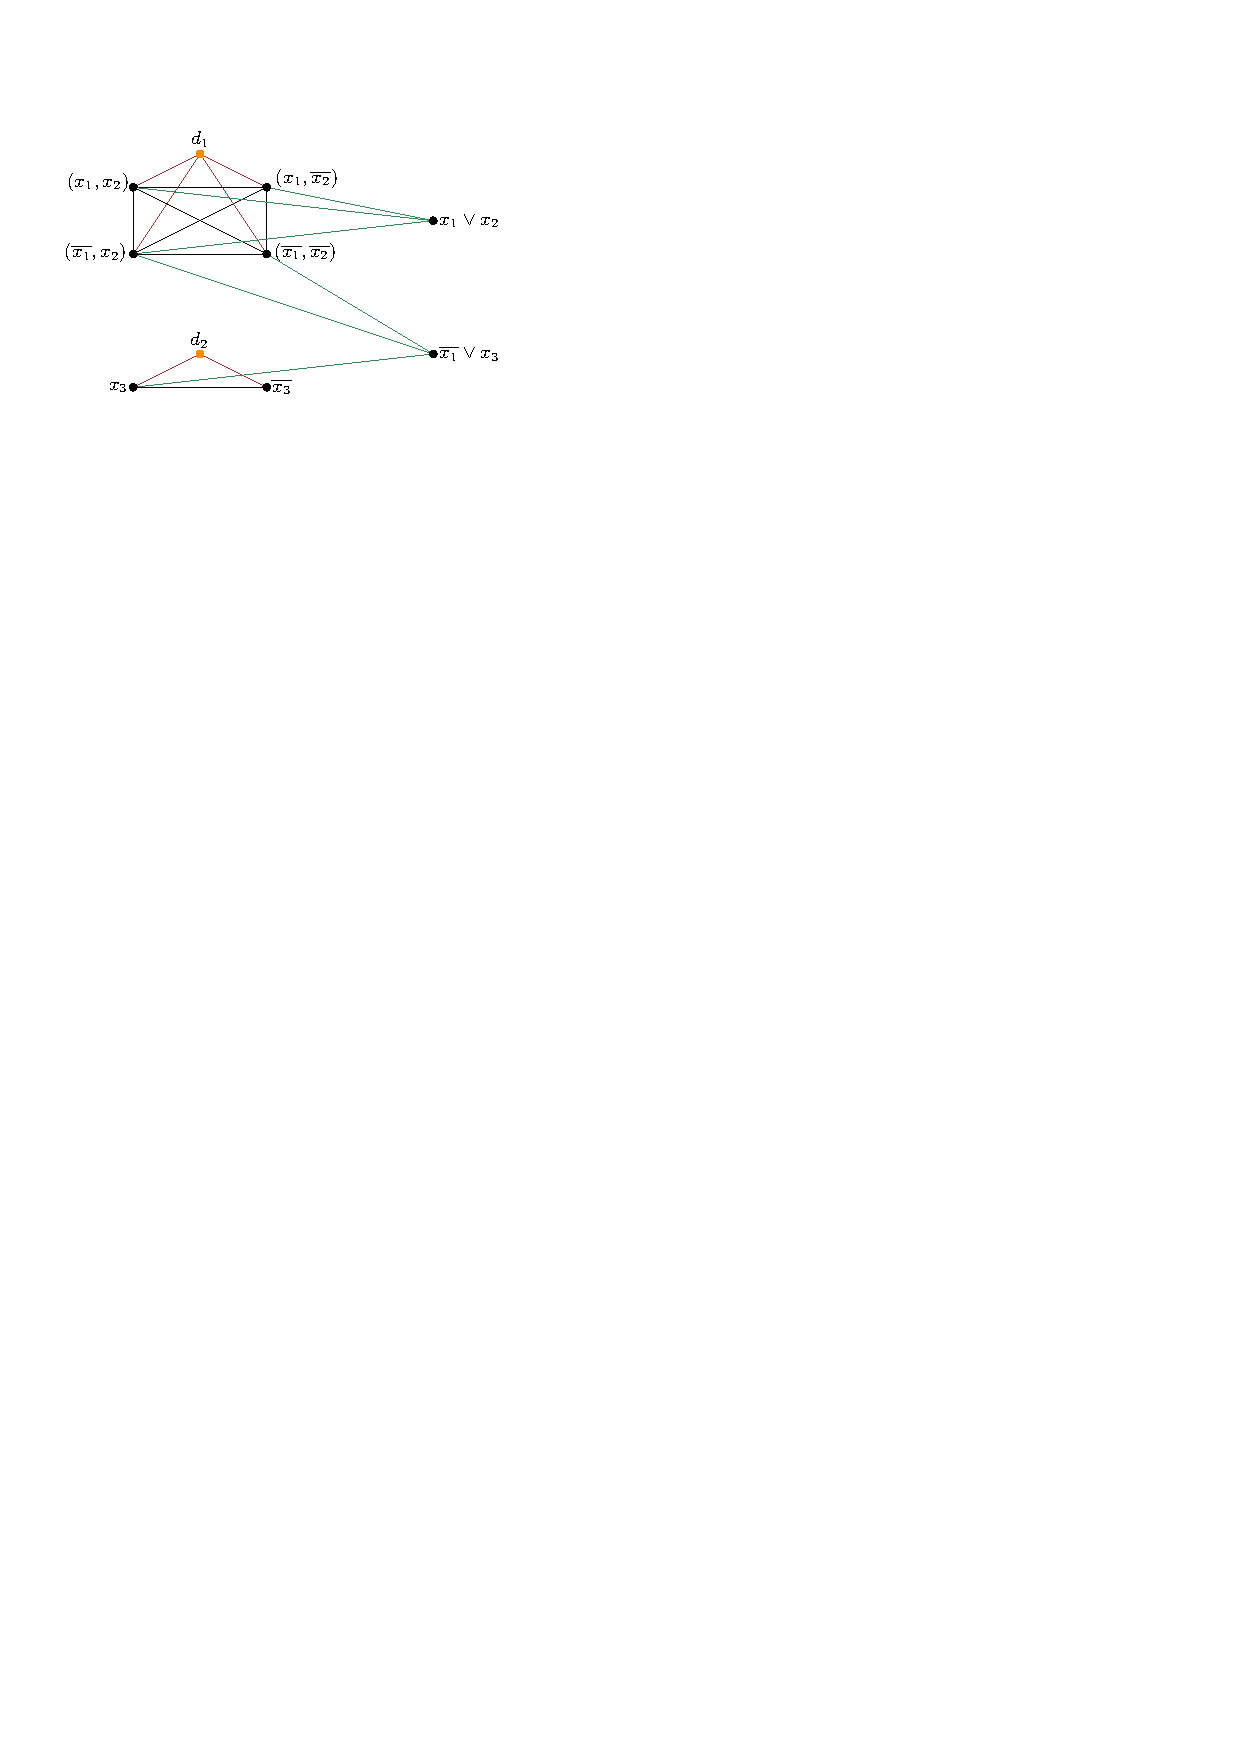
\includegraphics[scale = 1.2]{./images/reduction.pdf}
    \caption{Beispielkonstruktion der in \hyperref[oe:korollar:seth]{Korollar} \ref{oe:korollar:seth} beschriebenen Reduktion für $V = \{x_1, x_2, x_3\} $ und $ C = \{x_1 \lor x_2,\, \overline{x_1} \lor x_3\}$.}
    \label{OE:fig:reduction}
  \end{figure}

  \noindent
  Ist nun $I$ eine Ja-Instanz mit Wahrheitsbelegung $b: V \rightarrow \{t,\, f\}$, ergibt sich für $I'$ das folgende Dominating Set $M$:

  \noindent
  $M = \{(l_{i,1}, \dots, l_{i,q}) \,|\, b(l_{i,j}) = t\}$.
  Denn: Jede Wahrheitsbelegung ist in $G$ in jeweils genau einen Knoten aus verschiedenen Gadgets \enquote{aufgeteilt}. Durch die Konstruktionsvorschrift
  ist damit schonmal jedes Gadget dominiert. Da zusätzlich $b$ erfüllend ist, ist auch jeder Klauselknoten abgedeckt.

  \noindent
  Ist wiederum $I'$ eine lösende Instanz mit Dominating Set $M$, konstruieren wir eine Wahrheitsbelegung $b$ wie folgt:

  \vspace{0.25cm}
  Sei $b(x_{i,j}) = \begin{cases}
    t, & \text{falls}\ (l_{i,1}, \dots, x_{i,j}, \dots, l_{i,q}) \in M \\
    f, & \text{falls}\ (l_{i,1}, \dots, \overline{x_{i,j}}, \dots, l_{i,q}) \in M \; \lor \; d_i \in M
  \end{cases}$
  \vspace{0.25cm}

  \noindent
  Dabei gilt stets $(l_{i,1}, \dots, x_{i,j}, \dots, l_{i,q}) \in M$,  $(l_{i,1}, \dots, \overline{x_{i,j}}, \dots, l_{i,q}) \in M$ oder $d_i \in M$, da die
  Hinzunahme von Klauselknoten allein nicht ausreichen würde, um ein Dominating Set zu konstruieren.

  \noindent
  Damit reduziert sicht $p$-\textsc{CNF-SAT} auf $k$-\textsc{DominatingSet} wobei $V(G) \in \BigO{2^{\frac{n}{r}}}$.
  Dabei ist die Reduktion selbst dominiert durch Konstruktion der Kanten, die in $\BigO{|V(G)|^2} = \BigO{2^{2\frac{n}{r}}}$ realisiert werden kann. 

  \vspace{0.25cm}
  \noindent
  Angenommen, es existiert ein Algorithmus für $k$-\textsc{DominatingSet} mit Laufzeit in \BigO{|V(G)|^{k - \varepsilon}} für $\varepsilon < 1$.
  Dann ergibt sich im Widerspruch zur \hyperref[oe:definition:seth]{SETH} für $p$-\textsc{CNF-SAT} die Laufzeit:
  
  \begin{equation*}
    \begin{split}
     &  \BigO{2^{\frac{2n}{r}}} + \BigO{|V(G)|^{k - \varepsilon}} \\
     & = \BigO{2^{\frac{2n}{r}}} + \BigO{(2^{\frac{n}{r}})^{k - \varepsilon}} \\
    (k = r \geq 3,\,  \varepsilon < 1) &  = \BigO{(2^{\frac{n}{r}})^{k - \varepsilon}} \\ 
    & = \BigO{2^{\frac{nk}{r} - \frac{n\varepsilon}{r}}} \\
    &  = \BigO{2^{\frac{nk}{r} (1 - \frac{1}{k}\varepsilon)}} \\
    (\tilde{\varepsilon} := \frac{1}{k}\varepsilon < 1, k = r)  & = \BigO{2^{|V| (1 - \tilde{\varepsilon})}}
    \end{split}  
  \end{equation*}
\end{proof}

\subsection{Fazit und offene Fragen}

Parametrisierte Algorithmen sind ein relativ junges Teilgebiet der theoretischen Informatik. Durch Betrachtung eines zusätzlichen
Parameters ist es möglich, das Laufzeitverhalten von Algorithmen deutlich feingranularer zu untersuchen. Jedoch ist nicht klar,
welche Wahl des Parameters zur gewünschten Einsicht führt oder ob es überhaupt eine Wahl des Parameters gibt, die die gewünschte Einsicht ermöglicht.
Diese Ausarbeitung fokussierte sich auf die exakte Lösung von Problemen und deren parametrisierte Laufzeit. Mittels der
Problemkernreduktion wurde zudem eine alternative Sichtweise auf ein Problem als Komposition eines \enquote{schweren} und \enquote{leichten} Teils
geboten. Jedoch liefert die Problemkernreduktion selbst keine tiefergehende Begründung, warum bestimmte Teile einer Instanz Schwierigkeit hervorrufen.
Zusätzlich stellt sich die Frage nach parametrisierten Approximantionsalgorithmen und auch die Komplexitätstheorie wurde mit der
Problemklasse \FPT\xspace nur gestreift. Es seien hier zusätzlich die Problemklasse \XP\xspace und die \W-Hierarchie erwähnt.
\noindent
Schließlich wurden mit der ETH und SETH zwei Hypothesen vorgestellt, mit deren Hilfe sich Laufzeitabschätzungen ermöglichen
lassen, die mit denen von tatsächlich existierenden Algorithmen sehr gut übereinstimmen. Trotzdem bleibt die Frage nach Gültigkeit beider ungeklärt. Gültigkeit würde $\P \neq \NP$ implizieren. Es sei hier
erwähnt, das obwohl die ETH von vielen als gültig angesehen wird, das Meinungsbild bei der SETH gestreut ist \cite{Parameterized,Beyond}.% Bei Interesse sei auf (TODO: parameterized algos) verwiesen.




\bibliography{references}



%%%%% YOUR REPORT ENDS HERE




\end{document}
